%%%%%%%%%%%%%%%%%%%%%%%%%%%%%%%%%%%%%%%%%%%%%%%%%%%%%%%%%%%%%%%%%%%%%%%%%%%%%%%%
\section{Discussion}
\label{sec:discussion}

%%%%%%%%%%%%%%%%%%%%%%%%%%%%%%%%%%%%%%%%%%%%%%%%%%%%%%%%%%%%%%%%%%%%%%%%%%%%%%%%
\subsection{Proposed TR WPT System}
\label{sec:system}

This research represents a first step in the exploration of a WPT system based on TR. We now propose one possible proof-of-concept system in Fig.~\ref{fig:SysImage}. In this work, we investigate one particular performance parameter of the system. However, many unknowns regarding the design and performance of a complete system remain.

The proposed system has two basic components. The first is a rectenna that serves as the receiver. Although the system as described in Section~\ref{sec:meth} would require an out-of-band feedback channel between the receiver and transmitter, prior work has shown how a transmitter can target  receivers entirely in-band~\cite{nltr-wave-chaotic,roman}. Our system in Fig.~\ref{fig:SysImage} builds on these findings.

The second component is a transmitter that performs the time reversal process. This system will record identifying signals from the receiver(s), time reverse the signals, and re-broadcast them into the environment.

Although not a component of the system, another important consideration in building a WPT system based on TR is the environment, as TR is heavily dependent on environmental factors. A low-loss scattering environment is necessary for the technique to be effective.

\subsection{Contributions and Future Work}
\label{sec:contrib}

In the above experiments, we demonstrate the shape of the spatial profile of an electromagnetic
time reversed collapse. This profile takes the form \texttt{|sinc(x)|}, dependent on wavelength $b$.
Additionally, the ability of a TR system to transmit energy to a moving target is
demonstrated to be dependent on the spatial profile and transmission dead
time $t_{d}$.

Any WPT system utilizing time reversal will have to account for the
finite-size bubble of fields around the main reconstruction point.
Methods have been developed to improve the spatial focusing of reconstructions
well below the diffraction limit~\cite{lerosey-focusing}.

Based on the results shown in Fig.~\ref{fig:moving_recon}, it is clear that a faster
processing speed is required to track a moving target.
%
Nevertheless, we believe one of the main advantages of time reversal over
existing WPT methods is its ability to track moving
targets~\cite{fink,nltr-wave-chaotic}.


\begin{figure}[t]
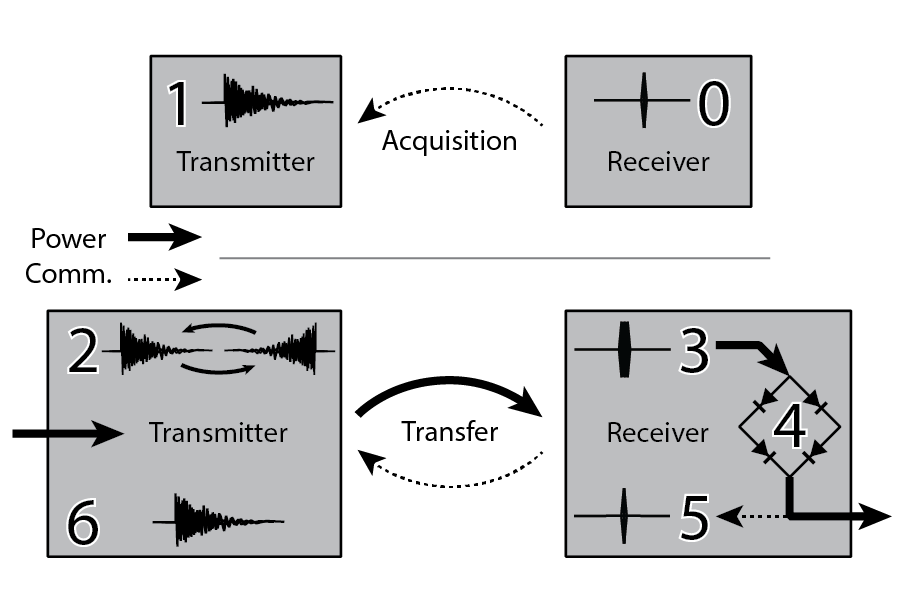
\includegraphics[width=\columnwidth]{figs/WPTSysAlt}
\caption{A notional time reversal wireless power transfer system. A new receiver joins the system by broadcasting or emitting a characteristic signal (0). Here, the receiver emits a signal, but it is also possible to detect it in other ways, as in~\cite{nltr-wave-chaotic}. In any case, the next sona that the transmitter collects will contain spatial information leading back to this receiver (1). In the power transfer cycle, the sona is time-reversed (2) and broadcast back into the environment. An amplified version of the signal reconstructs on the receiver (3), which rectifies the energy (4). A small amount of the energy is used to broadcast a new signal (5) into the environment, which will be collected in the next sona (6). The cycle repeats from (2).}
\label{fig:SysImage}
\end{figure}
%%%%%%%%%%%%%%%%%%%%%%%%%%%%%%%%%%%%%%%%%%%%%%%%%%%%%%%%%%%%%%%%%%%%%%%%%%%%%%%%

%%%%%%%%%%%%%%%%%%%%%%%%%%%%%%%%%%%%%%%%%%%%%%%%%%%%%%%%%%%%%%%%%%%%%%%%%%%%%%%%
\subsection{Limitations}
\label{sec:limitations}


These experiments were limited primarily by the environment and equipment used
for testing.
%
A consumer electronics environment is likely to be much larger than the chamber
used in this study, and filled with clutter.
%
Both of these properties would improve the modal density of the environment,
creating more transmission channels between source and target, ultimately
improving reconstruction quality.
%
On the other hand, such environments would likely have significantly larger loss
than those considered in our experiments. We found that approximately \ph{X}\% of energy transmitted through our test cavity was lost due to absorption. Understanding and characterizing how environmental factors impact TR is a major obstacle to the design of a TR WPT system. Environmental effects should be a major research priority accordingly.

%Our results show that time reversal mirrors may be able to effectively
%exploit multiple channels, but we leave this to future work.
%Great benefit can also be achieved by utilizing multi-channel time reversal mirrors.
%Understanding how
%to maximize the effectiveness of these technologies while minimizing cost is
%critical.

The single-channel time reversal method is limited in the amount of power it can
transmit to a target.
%
It is certainly sufficient to perform long-term trickle charging or to act as a
secondary-source of energy extending battery life.
%
A multi-channel realization of time reversal will be able to deliver much
greater time-integrated power.



The theoretical limit for the speed of the time reversal process needs to be
determined.
%
These experiments were severely limited by the processing time of the combined
MATLAB-DSO-AWG-PSG test and measurement system.
%
Dedicated hardware and firmware would eliminate communication overhead and thus
dramatically improve the speed of the WPT process presented here.
%%%%%%%%%%%%%%%%%%%%%%%%%%%%%%%%%%%%%%%%%%%%%%%%%%%%%%%%%%%%%%%%%%%%%%%%%%%%%%%%
